\begin{figure}[t]
\begin{centering}
\caption{Crop choice changes in response to a \$10 groundwater tax}
\label{fig:cf_water_tax}
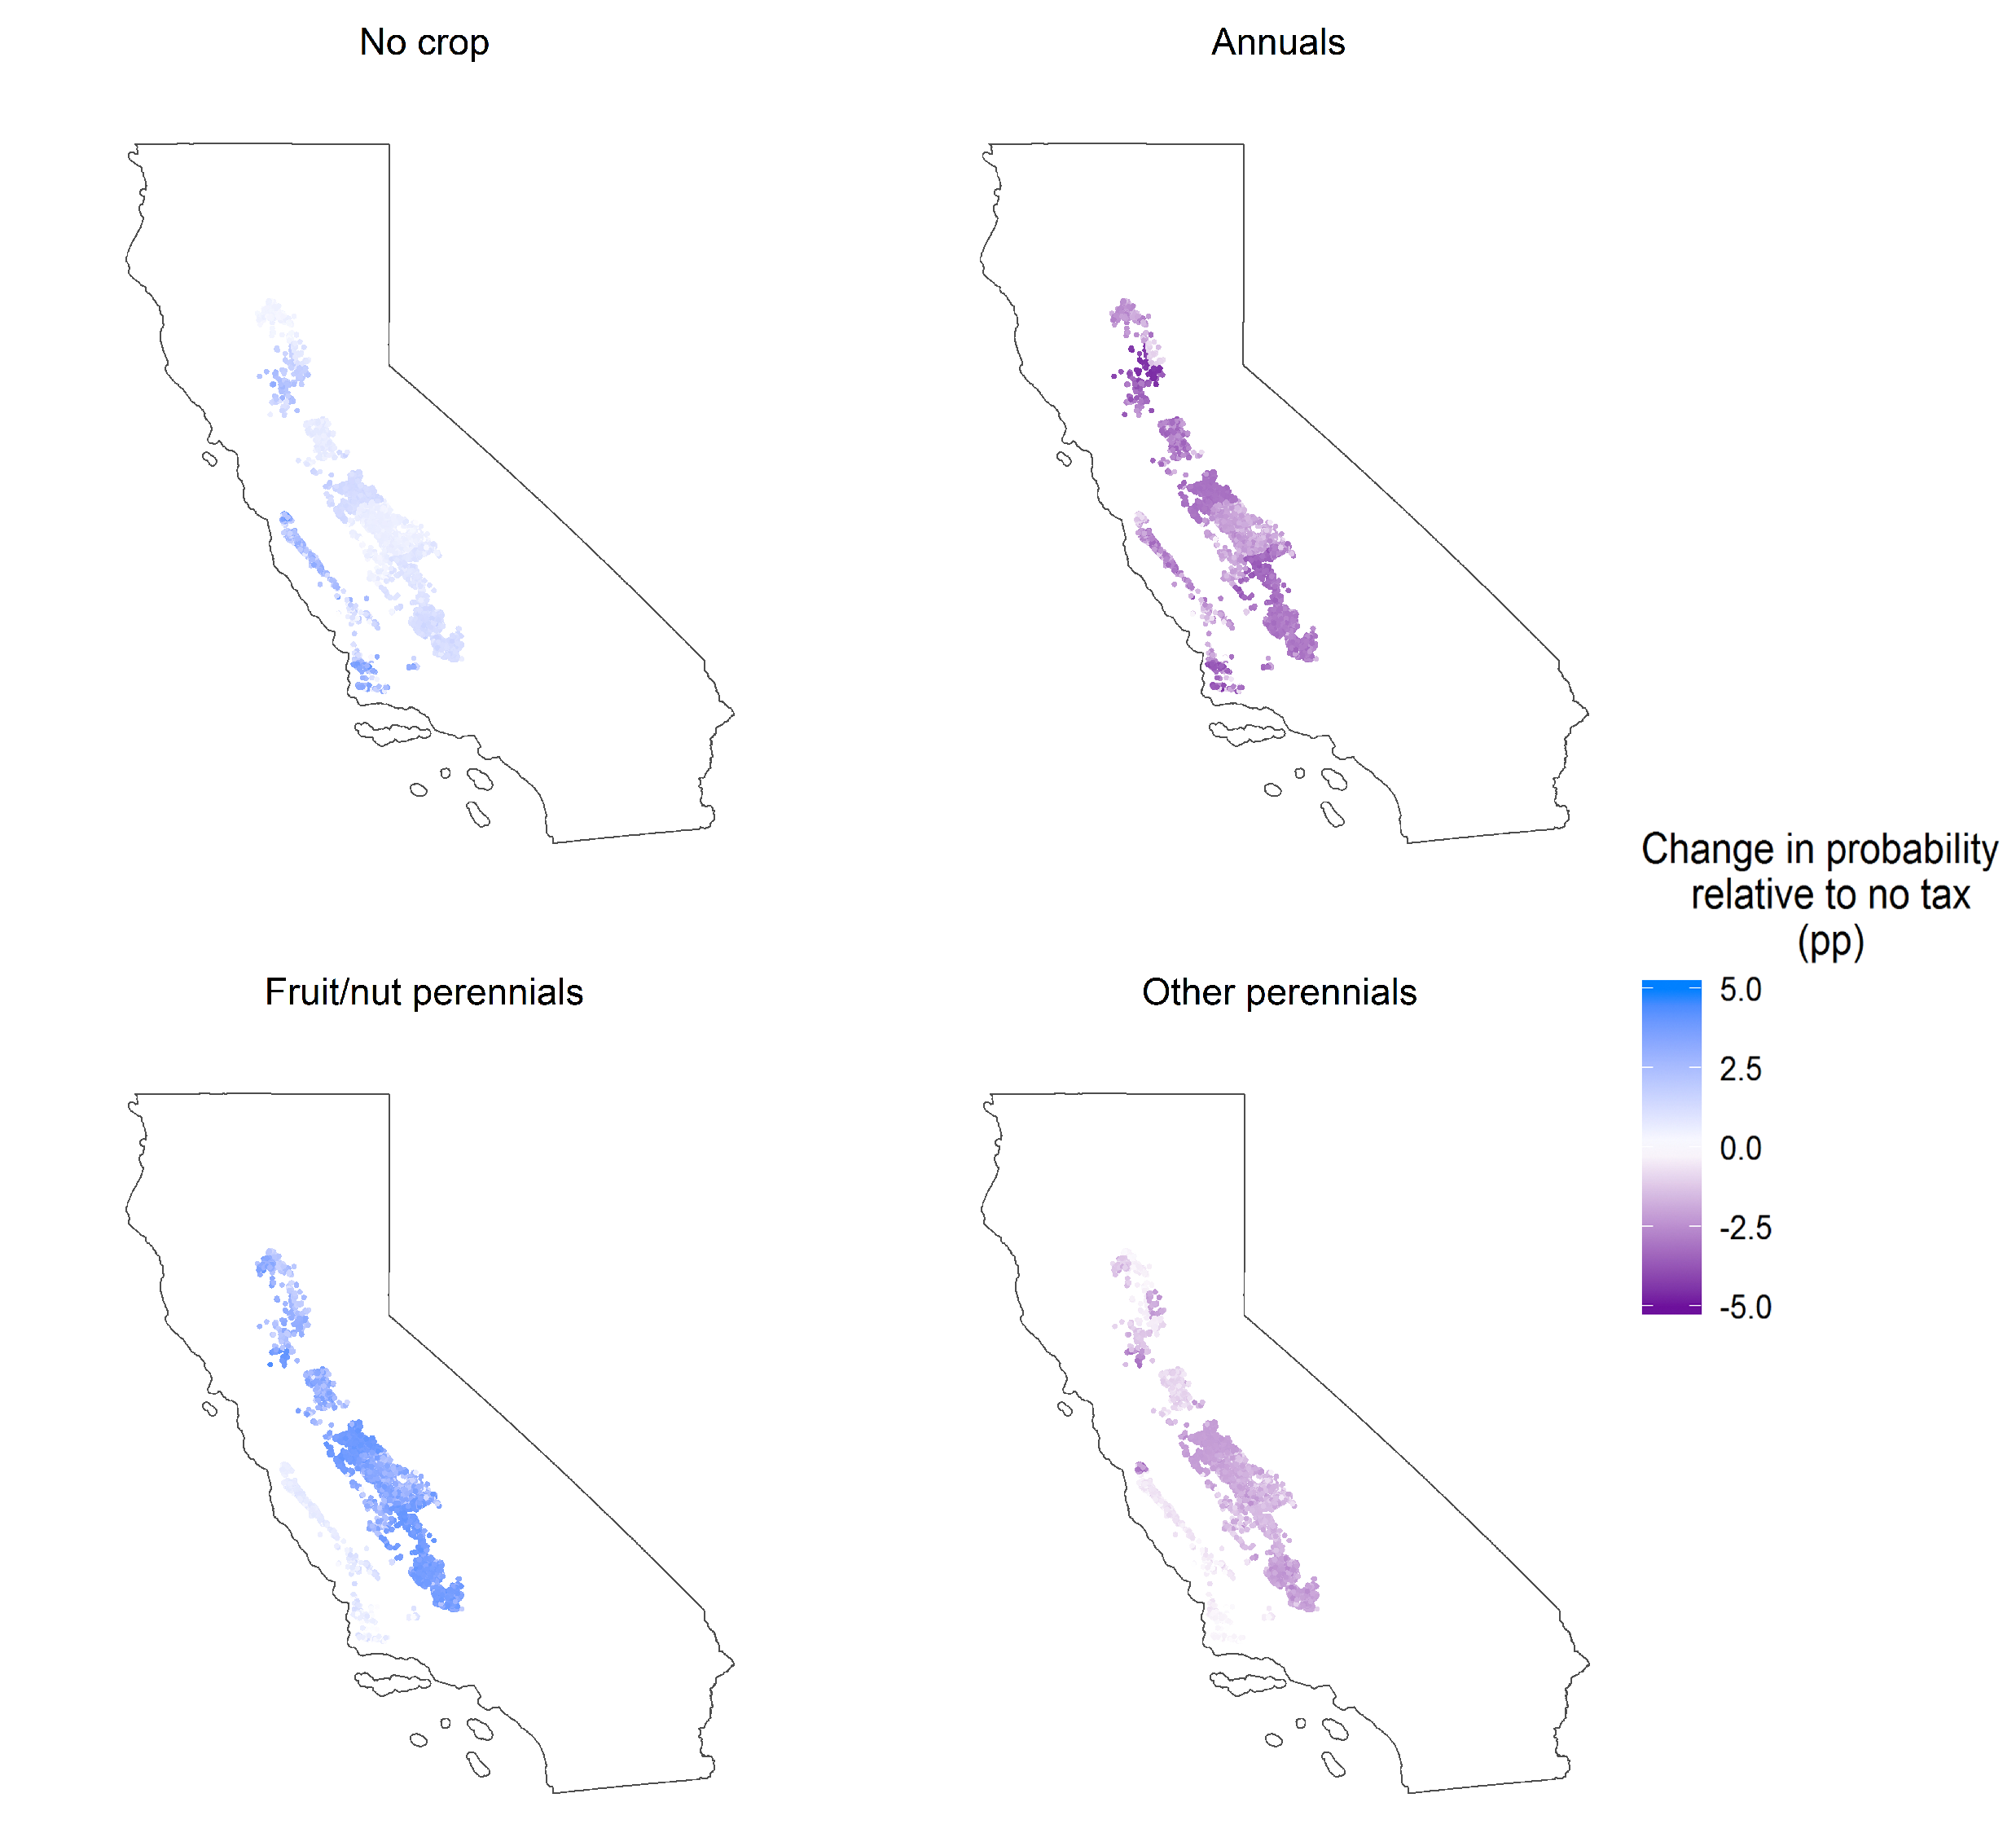
\includegraphics[width=\textwidth]{Figures/clu_prob_10tax_fullstate_combined.pdf}
\caption*{\scriptsize \emph{Notes:} This figure plots the estimated counterfactual changes in crop choice resulting from a \$10 groundwater tax, relative to no tax. Each dot is the centroid of a CLU in our sample. To generate these estimates, we first compute the average probability each CLU farms each crop type across all sample years in the no-tax baseline. We then compute similar probabilities with the groundwater price increased by \$10 per acre-foot. Finally, we subtract the no-tax baseline from the \$10 tax counterfactual to compute the change in probability of having each land type. The top left panel shows the change in fallowing. The top right panel shows the change in annual crops. The bottom left panel shows the change in fruit and nut perennials, and the bottom right shows changes in other perennials.
}
\end{centering}
\end{figure}
